% PGF/TikZ manual (TeX Live 2025), pgfmanual-en-library-plot-handlers.tex,
% "Constant Plot Handlers": the examples for \pgfplothandlerconstantlineto,
% \pgfplothandlerconstantlinetomarkright and \pgfplothandlerconstantlinetomarkmid
% all stream (0cm,0cm), (1cm,1cm), (2cm,0.5cm). Here the same points use
% the ordinary TikZ keys from pgfmanual-en-tikz-plots.tex, without node labels.
% Panel offsets (0, 2.5, 5cm) are included in the coordinates, not a transform.
% From left to right: blue steps at x=1,2; teal at x=0,1; red at x=.5,1.5
% (local cm). All changes of height are connected by vertical strokes.
\documentclass[border=2pt]{standalone}
\usepackage{tikz}
\begin{document}
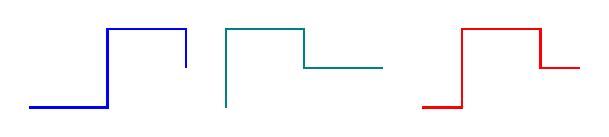
\begin{tikzpicture}
  \draw[blue,thick] plot[const plot] coordinates {(0,0) (1,1) (2,0.5)};
  \draw[teal,thick] plot[const plot mark right] coordinates {(2.5,0) (3.5,1) (4.5,0.5)};
  \draw[red,thick] plot[const plot mark mid] coordinates {(5,0) (6,1) (7,0.5)};
\end{tikzpicture}
\end{document}
